% =============================================================================
% =  My Idea (2 pages)
% =============================================================================

\section{The Impact of Structural Quality} \label{sectionMyIdea}

% --- Understand Software Maintenance -----------------------------------------
\subsection{Software Maintenance} \label{subSoftwareMaintenance}

The structural quality of a software system will impact the software evolution. If the project has poor structural quality, its ability to evolve will be minimized, and the software system will eventually ``die-off'' so to speak.

There is much planning involved in all software creation projects in what the product will be, will do, who it is for, etc. One of the things that should also be on the planning list is long-term maintenance and growth. That is, how do we build a thing that will be easier to add features to down the road?

Let us define maintainability in the context of software. For example, a system would be considered easy to maintain if it is easy to debug and easy to add new features. These new features are generally considered minor features, and may often be reported as bugs by users, when in reality, they are looking for functionality enhancements \cite{wiki:software-maintenance}.

\vspace{0.25cm}
\begin{displayquote}
``Software maintenance in software engineering is the modification of a software product after delivery to correct faults, to improve performance or other attributes.'' \cite{wiki:software-maintenance}
\end{displayquote}
\vspace{0.25cm}

It may be easier to understand what characteristics define a system with poor maintainability. These types of systems will have poor code quality, leading to defects. For example, there could be undetected vulnerabilities or vulnerabilities that have been ignored. It may be that the system is overly complex. In addition to the complexity, it could be hard to read due to poor naming or dead (unused) code throughout the source code.

A project is known to have good maintainability when there is an enforced set of clean and consistent standards for the code. This often involves having human-readable names for functions, methods, and variables. Any complex code is minimized, and methods are small and focus on a single thing. Parts of the system are decoupled and organized, making it easy to work on different parts with low impact on unrelated parts. For example, the code is DRY (there is limited redundancy in the code), unused code has been removed, and there is a level of documentation that supports an easy understanding of the system.

Why should we care about whether the code is maintainable? It is assumed that a large amount of the cost over the lifetime of a project is attributed to maintainability. Fred Brooks, in his book ``The Mythical Man-Month'' even claimed that over 90\% of the costs for a typical software system come up in the maintenance phase \cite{brooks:mythical}. Once the bulk of the system is off the ground and live worldwide, how well the team can improve the system with new features and fix bugs, even working on different parts in parallel, can be impacted by its maintainability. Any successful piece of software will inevitably need to be maintained.

% --- Understand Software Evolution -------------------------------------------
\subsection{Software Evolution} \label{subSoftwareEvolution}

There is a distinction to be made between \textbf{software maintenance} and \textbf{software evolution}. We will refer to software maintenance as bug resolution and for minor functional improvements. For example, we can consider this routine maintenance when we must fix a broken route in the application or provide a subtle enhancement on the user experience. However, when we look at upgrades to the system, adaptations to the changing and growing needs of the user, or migrating the system to a new technology, we can refer to this as evolution of the software.

The evolution of software can result from new laws that have come into being. As technology itself changes, governing bodies must continually revisit data collection and information sharing policies. Changes in technology and laws may lead to adaptations in the software systems.

It is also fair to say that systems will change because we can never fully determine a user's needs at the start of a project. It would be safe to say that the user's needs will change over time themselves. This leads to a never-ending project that will always need some form of enhancement.

Meir ``Manny'' Lehman and László ``Les'' Bélády contributed to a list of laws involving software evolution known as Lehman's Laws that describe a balance between forces that drive new developments while also slowing progress. These laws apply to programs that were written to perform some real-world activity, where its behavior is linked to the environment in which it runs; additionally, this program category assumes that the program needs to adapt to varying requirements and circumstances in that environment. Eight laws were created and are listed below. \cite{wiki:lehmans-laws}

\todo{TODO: Read and reference ``An Empirical Study of Lehman’s Law on Software Quality Evolution'' \cite{yu:2013}}.

\vspace{0.25cm}
\begin{enumerate}
    % "Continuing Change" — an E-type system must be continually adapted or it becomes progressively less satisfactory.
    \item \textbf{Continuing Change} \textit{(1974)}
    
    % "Increasing Complexity" — as an E-type system evolves, its complexity increases unless work is done to maintain or reduce it.
    \item \textbf{Increasing Complexity} \textit{(1974)}

    % "Self Regulation" — E-type system evolution processes are self-regulating with the distribution of product and process measures close to normal.
    \item \textbf{Self Regulation} \textit{(1974)}

    % "Conservation of Organisational Stability (invariant work rate)" — the average effective global activity rate in an evolving E-type system is invariant over the product's lifetime.
    \item \textbf{Conservation of Organisational Stability} \textit{(1978)}

    % "Conservation of Familiarity" — as an E-type system evolves, all associated with it, developers, sales personnel, and users, for example, must maintain mastery of its content and behavior to achieve satisfactory evolution. Excessive growth diminishes that mastery. Hence the average incremental growth remains invariant as the system evolves.
    \item \textbf{Conservation of Familiarity} \textit{(1978)}

    % "Continuing Growth" — the functional content of an E-type system must be continually increased to maintain user satisfaction over its lifetime.
    \item \textbf{Continuing Growth} \textit{(1991)}

    % "Declining Quality" — the quality of an E-type system will appear to be declining unless it is rigorously maintained and adapted to operational environment changes.
    \item \textbf{Declining Quality} \textit{(1996)}

    % "Feedback System" (first stated 1974, formalised as law 1996) — E-type evolution processes constitute multi-level, multi-loop, multi-agent feedback systems and must be treated as such to achieve significant improvement over any reasonable base.
    \item \textbf{Feedback System} \textit{(1996)}
\end{enumerate}
\vspace{0.25cm}

The first law, ``Continuing Change,'' tells us that if a system does not adapt, it will become progressively less satisfactory. The second, ``Increasing Complexity,'' explains that as a system evolves, unless work is done to maintain or reduce complexity, the complexity will increase. This can be due to the added volume of the code from new features or even an increasing number of developers that have edited the code. Unless this phenomenon of increased complexity is actively addressed during changes, it can impact the maintainability (and the ability of a project to continue evolving) in the future.

Lehman's fifth law, ``Conservation of Familiarity,'' explains how the average incremental growth does not change over time as a system evolves. The people interacting with the system, such as the developers, business persons, or users, must still continue using and working within the system at the same ``level of mastery.'' If the system grows and changes excessively, the mastery will drop, slowing down the next set of changes. This could be because the source code or architecture has become more complex (impacting the developers' ability to adapt and enhance the system) or because the user features have changed so that the system audience needs time to master the new interfaces or new tools. Because of this natural ``slow-down'' for excessive change, the average incremental growth will remain steady. We can see a simplified visual in ``Fig.~\ref{figConservationOfFamiliarity}'' showing that when the number of changes spikes (that is to say, when there is excessive growth in a system), it will be followed by an iteration of fewer changes, leading to a nearly consistent average of incremental growth (the thick, horizontal line) over time.

\begin{figure}[ht]
    \centerline{
        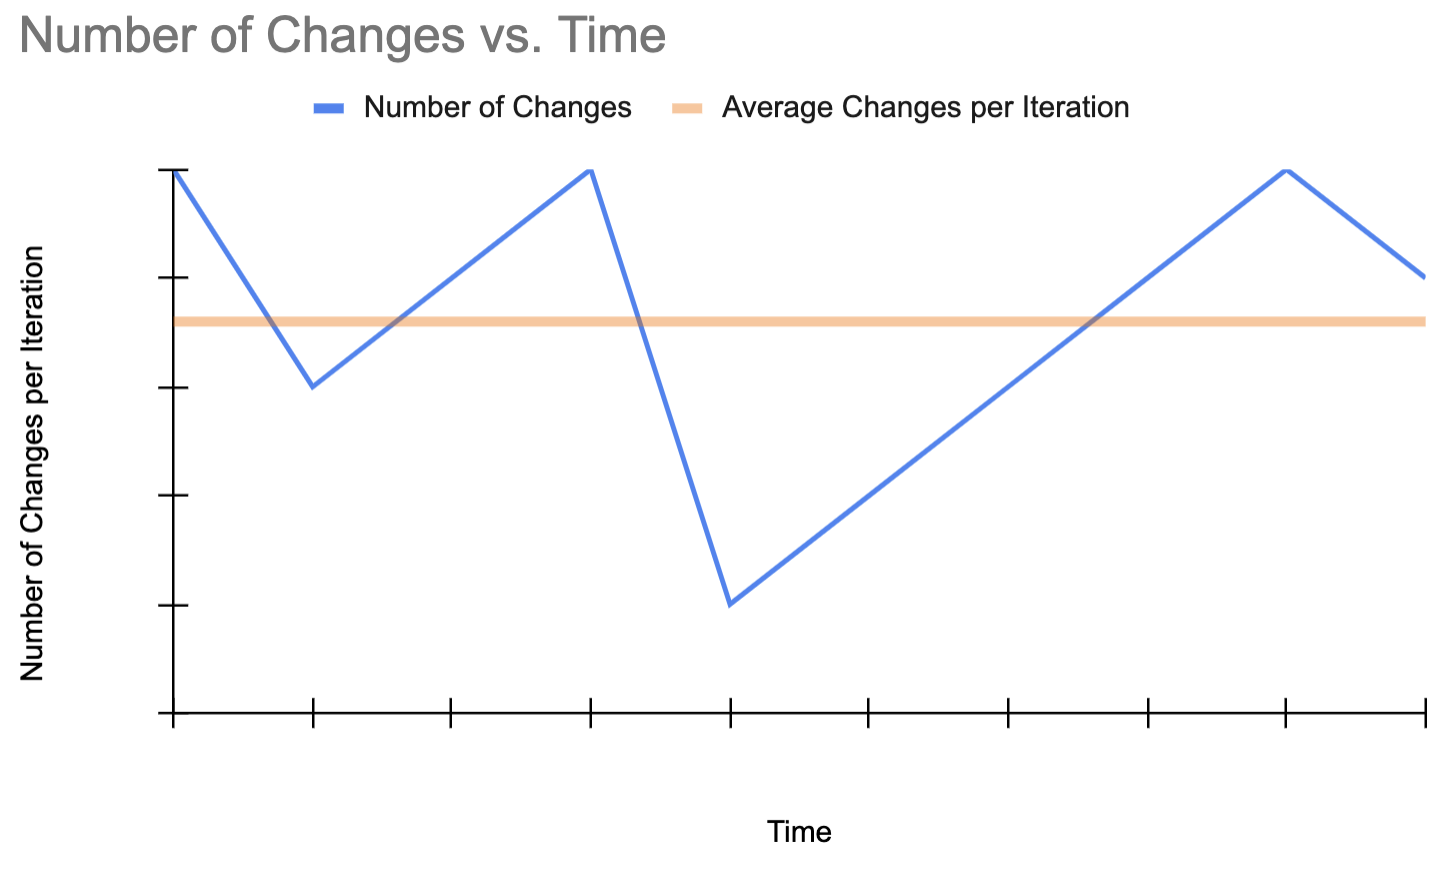
\includegraphics[width=\columnwidth]{Changes-vs-Time}
    }
    \caption{A simplified visual of Lehman's fifth law, ``Conservation of Familiarity.''}
    \label{figConservationOfFamiliarity}
\end{figure}

In Lehman's sixth law, ``Continuing Growth,'' we see that the system user's satisfaction will not be maintained without continually increasing the functional content. Along a similar idea, the law pertaining to ``Declining Quality'' states that if the operational environment for the system does not change, the system's quality will appear to decline. Yu and Mishra performed focused research on supporting Lehman's Laws, especially in the case of the seventh law pertaining to declining quality, by defining a metric for software quality and reviewing the bug history, growth of size, complexity, and quality of two large open-source systems \cite{yu:2013}. Therefore, we must continue adapting for even the appearance of the maintained quality of a system.

With all of these characteristics surrounding the evolution of software, we benefit from the Internet that has positively improved the experience. Two common resources currently available to developers have impacted software evolution \cite{wiki:software-evolution}:

\vspace{0.25cm}
\begin{enumerate}
    \item The rapid growth of the World Wide Web and Internet Resources make it easier for users and engineers to find related information.
    \item Open source development where anybody could download the source codes and modify it has enabled fast and parallel evolution (through forks).
\end{enumerate}
\vspace{0.25cm}

These two suggestions are very evident in modern development. For example, a developer may regularly use resources like StackOverflow to find solutions to problems and use open-source tools that the developer and their team can contribute to or adjust to their specific needs.

\subsection{Measuring Maintainability} \label{subMeasureMaintainability}

Despite the nuanced differences between \textit{maintainability} and \textit{evolution}, the two characteristics run parallel to each other. If a system is easy to maintain, it will also be easier to evolve. If we can measure our system's maintainability, we can also determine if our system is in a good position to continue evolving to meet our future needs.

Several tools attempt to provide some value around these ideas. In this paper, we will focus on the metrics that Pylint provides, specifically looking into the Refactor score of Pylint.

We will look at many open-source Python systems using Pylint and attempt to correlate the data from the Pylint scores to the level of ease in adding new features to the system. This will determine if a system is more maintainable with better Pylint scores. 

\todo{FUTURE EDITION: To do this, we will measure the locality of the changes by the number of files that are edited in a commit. We will also focus on commits that represent new features, not on commits that are bug fixes.}
